\section{Line\-Iterator Class Reference}
\label{classLineIterator}\index{LineIterator@{LineIterator}}
{\tt \#include $<$lineiterator.hpp$>$}

Inheritance diagram for Line\-Iterator::\begin{figure}[H]
\begin{center}
\leavevmode
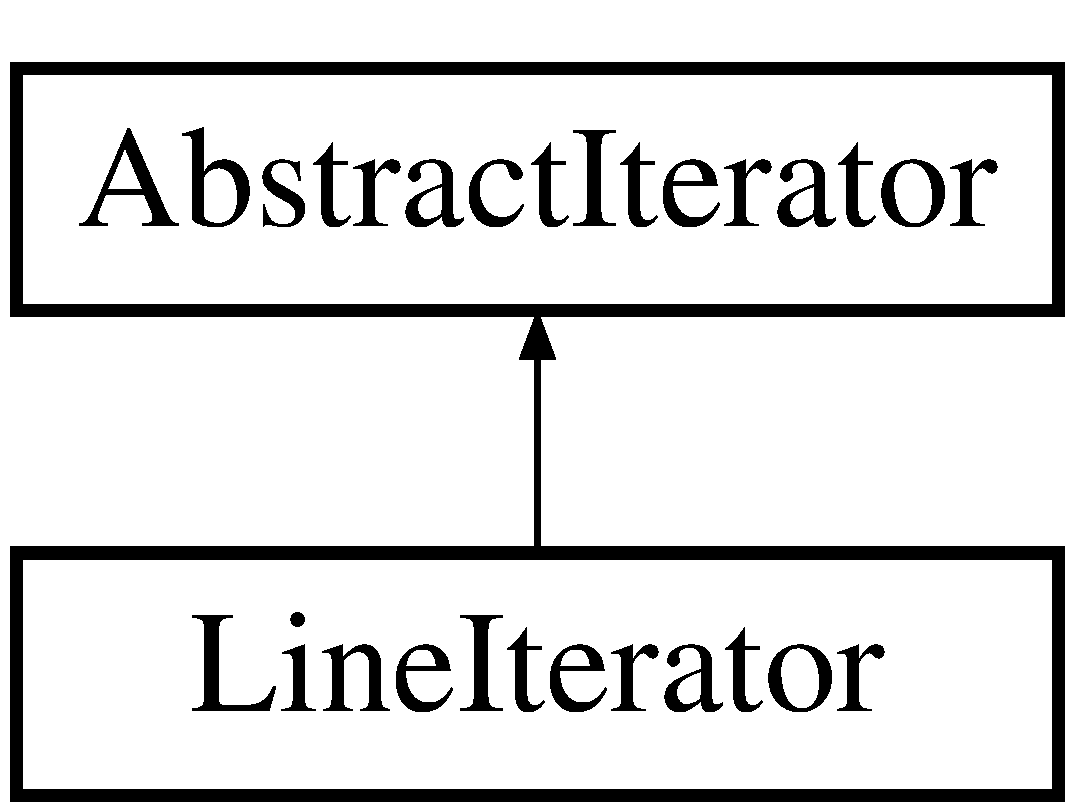
\includegraphics[height=2cm]{classLineIterator}
\end{center}
\end{figure}
\subsection*{Public Member Functions}
\begin{CompactItemize}
\item 
{\bf Line\-Iterator} (int x1, int y1, int x2, int y2)
\item 
virtual bool {\bf operator!} ()
\item 
virtual void {\bf operator++} (int)
\item 
int {\bf x} ()
\item 
int {\bf y} ()
\end{CompactItemize}
\subsection*{Protected Attributes}
\begin{CompactItemize}
\item 
int {\bf \_\-x1}
\item 
int {\bf \_\-x2}
\item 
int {\bf \_\-y1}
\item 
int {\bf \_\-y2}
\item 
int {\bf \_\-param}
\item 
int {\bf \_\-max}
\item 
int {\bf \_\-lastx}
\item 
int {\bf \_\-lasty}
\item 
int {\bf \_\-x}
\item 
int {\bf \_\-y}
\end{CompactItemize}


\subsection{Constructor \& Destructor Documentation}
\index{LineIterator@{Line\-Iterator}!LineIterator@{LineIterator}}
\index{LineIterator@{LineIterator}!LineIterator@{Line\-Iterator}}
\subsubsection{\setlength{\rightskip}{0pt plus 5cm}{\bf Line\-Iterator} (int {\em x1}, int {\em y1}, int {\em x2}, int {\em y2})}\label{classLineIterator_a0}




\subsection{Member Function Documentation}
\index{LineIterator@{Line\-Iterator}!operator"!@{operator"!}}
\index{operator"!@{operator"!}!LineIterator@{Line\-Iterator}}
\subsubsection{\setlength{\rightskip}{0pt plus 5cm}bool operator! ()\hspace{0.3cm}{\tt  [virtual]}}\label{classLineIterator_a1}




Implements {\bf Abstract\-Iterator} {\rm (p.\,\pageref{classAbstractIterator_a0})}.\index{LineIterator@{Line\-Iterator}!operator++@{operator++}}
\index{operator++@{operator++}!LineIterator@{Line\-Iterator}}
\subsubsection{\setlength{\rightskip}{0pt plus 5cm}void operator++ (int)\hspace{0.3cm}{\tt  [virtual]}}\label{classLineIterator_a2}




Implements {\bf Abstract\-Iterator} {\rm (p.\,\pageref{classAbstractIterator_a1})}.\index{LineIterator@{Line\-Iterator}!x@{x}}
\index{x@{x}!LineIterator@{Line\-Iterator}}
\subsubsection{\setlength{\rightskip}{0pt plus 5cm}int x ()}\label{classLineIterator_a3}


\index{LineIterator@{Line\-Iterator}!y@{y}}
\index{y@{y}!LineIterator@{Line\-Iterator}}
\subsubsection{\setlength{\rightskip}{0pt plus 5cm}int y ()}\label{classLineIterator_a4}




\subsection{Member Data Documentation}
\index{LineIterator@{Line\-Iterator}!_lastx@{\_\-lastx}}
\index{_lastx@{\_\-lastx}!LineIterator@{Line\-Iterator}}
\subsubsection{\setlength{\rightskip}{0pt plus 5cm}int {\bf \_\-lastx}\hspace{0.3cm}{\tt  [protected]}}\label{classLineIterator_p6}


\index{LineIterator@{Line\-Iterator}!_lasty@{\_\-lasty}}
\index{_lasty@{\_\-lasty}!LineIterator@{Line\-Iterator}}
\subsubsection{\setlength{\rightskip}{0pt plus 5cm}int {\bf \_\-lasty}\hspace{0.3cm}{\tt  [protected]}}\label{classLineIterator_p7}


\index{LineIterator@{Line\-Iterator}!_max@{\_\-max}}
\index{_max@{\_\-max}!LineIterator@{Line\-Iterator}}
\subsubsection{\setlength{\rightskip}{0pt plus 5cm}int {\bf \_\-max}\hspace{0.3cm}{\tt  [protected]}}\label{classLineIterator_p5}


\index{LineIterator@{Line\-Iterator}!_param@{\_\-param}}
\index{_param@{\_\-param}!LineIterator@{Line\-Iterator}}
\subsubsection{\setlength{\rightskip}{0pt plus 5cm}int {\bf \_\-param}\hspace{0.3cm}{\tt  [protected]}}\label{classLineIterator_p4}


\index{LineIterator@{Line\-Iterator}!_x@{\_\-x}}
\index{_x@{\_\-x}!LineIterator@{Line\-Iterator}}
\subsubsection{\setlength{\rightskip}{0pt plus 5cm}int {\bf \_\-x}\hspace{0.3cm}{\tt  [protected]}}\label{classLineIterator_p8}


\index{LineIterator@{Line\-Iterator}!_x1@{\_\-x1}}
\index{_x1@{\_\-x1}!LineIterator@{Line\-Iterator}}
\subsubsection{\setlength{\rightskip}{0pt plus 5cm}int {\bf \_\-x1}\hspace{0.3cm}{\tt  [protected]}}\label{classLineIterator_p0}


\index{LineIterator@{Line\-Iterator}!_x2@{\_\-x2}}
\index{_x2@{\_\-x2}!LineIterator@{Line\-Iterator}}
\subsubsection{\setlength{\rightskip}{0pt plus 5cm}int {\bf \_\-x2}\hspace{0.3cm}{\tt  [protected]}}\label{classLineIterator_p1}


\index{LineIterator@{Line\-Iterator}!_y@{\_\-y}}
\index{_y@{\_\-y}!LineIterator@{Line\-Iterator}}
\subsubsection{\setlength{\rightskip}{0pt plus 5cm}int {\bf \_\-y}\hspace{0.3cm}{\tt  [protected]}}\label{classLineIterator_p9}


\index{LineIterator@{Line\-Iterator}!_y1@{\_\-y1}}
\index{_y1@{\_\-y1}!LineIterator@{Line\-Iterator}}
\subsubsection{\setlength{\rightskip}{0pt plus 5cm}int {\bf \_\-y1}\hspace{0.3cm}{\tt  [protected]}}\label{classLineIterator_p2}


\index{LineIterator@{Line\-Iterator}!_y2@{\_\-y2}}
\index{_y2@{\_\-y2}!LineIterator@{Line\-Iterator}}
\subsubsection{\setlength{\rightskip}{0pt plus 5cm}int {\bf \_\-y2}\hspace{0.3cm}{\tt  [protected]}}\label{classLineIterator_p3}




The documentation for this class was generated from the following files:\begin{CompactItemize}
\item 
{\bf lineiterator.hpp}\item 
{\bf lineiterator.cpp}\end{CompactItemize}
